%% LaTeX template for FZI designed Document
%% by Matthias Huber and Florian Kuhnt
%%
%% version 0.4
%%
%% Problems, bugs and comments to
%% huber@fzi.de

\documentclass[parskip=true]{scrartcl}


% Toggle the following two lines to switch between english and german layout
%\usepackage[english]{babel} % English
\usepackage[ngerman]{babel} % Neue deutsche Rechtschreibung und Silbentrennung.

%\usepackage{templates/theme}

\usepackage{lipsum}
\usepackage{todonotes}	
\usepackage[nolist,nohyperlinks]{acronym}

\newboolean{titel} 
\setboolean{titel}{true}
\newboolean{inhalt} 
\setboolean{inhalt}{true}
\newboolean{headfoot} 
\setboolean{headfoot}{true}

% Dokumentangaben
\newcommand{\dokumenttitel}{[GA]}
\newcommand{\untertitel}{[Untertitel]}
\newcommand{\version}{0.1}
\newcommand{\veroeffentlichung}{1.1.1970}
\newcommand{\autor}{[Chrisitian Heinzmann]}
\newcommand{\validfrom}{1.1.1970}
\newcommand{\state}{-vertraulich-}

%Titelseite?
%\setboolean{titel}{false} 
%Inhaltsverzeichnis?
%\setboolean{inhalt}{false}
%FZI Kopf- und Fußzeile?
%\setboolean{headfoot}{false}

%Inhaltsverzeichnis?
%\setboolean{inhalt}{false}
%FZI Kopf- und Fußzeile?
%\setboolean{headfoot}{false}

\begin{document}

%Seiten ohne Kopf- und Fußzeile sowie Seitenzahl
\pagestyle{empty}

\begin{center}
\begin{tabular}{p{\textwidth}}


\begin{center}

\includegraphics[scale=0.4]{img/Hska_logo.png}
\end{center}


\\

\begin{center}
\LARGE{\textsc{
Genetische Algorithmen zur Optimierung von Hyperparametern eines k"unstlichen neuronalen Netzes\\
}}
\end{center}

\\


\begin{center}
\large{Fakult"at f"ur Maschinenbau und Mechatronik \\
der Hochschule Karlsruhe \\
Technik und Wirtschaft \\}
\end{center}

\\

\begin{center}
\textbf{\Large{Bachelorarbeit}}
\end{center}


\begin{center}
vom 01.03.2018 bis zum 31.08.2018 \\
vorgelegt von
\end{center}

\begin{center}
\large{\textbf{Christian Heinzmann}} \\
\small{geboren am 18.02.1995 in Heilbronn} \\
\small{Martrikelnummer: 52550}
\end{center}

\begin{center}
\large{Winter Semester 2019}
\end{center}

\\

\\

\begin{center}
\begin{tabular}{lll}
\textbf{Professor} & & Prof. Dr.-Ing. habil. Burghart\\
\textbf{Co-Professor} & & Prof. Dr.-Ing. Olawsky\\
\textbf{Betreuer FZI:} & & M. Sc. Kohout\\
\end{tabular}
\end{center}

\end{tabular}
\end{center}

\addsec{Eigenständigkeitserklärung und Hinweis auf verwendete
Hilfsmittel}
\label{erklaerung}

Eigenständigkeitserklärung und Hinweis auf verwendete
Hilfsmittel.
Hiermit bestätige ich, dass ich den vorliegenden Praxissemesterbericht selbständig
verfasst und keine anderen als die angegebenen Hilfsmittel benutzt habe. Die Stellen
des Berichts, die dem Wortlaut oder dem Sinn nach anderen Werken entnommen sind,
wurden unter Angabe der Quelle kenntlich gemacht.\\
\\[1.5cm]
Datum:	\hrulefill\enspace Unterschrift: \hrulefill
\\[3.5cm]

\addsec{Danksagungen}
\label{danksagungen}
An dieser Stelle möchte ich mich zuerst bei dem Forschungszentrum Informatik bedanken, durch die ich die
Möglichkeit bekommen habe, mich in einem innovativen Forschungszentrum auf meiner persönlichen und fachlichen Ebene weiter zu entwickeln.
Außerdem bedanke ich mich bei sämtlichen Kollegen der Abteilung Embedded Systems and Sensors Engineering, die
mich jederzeit hilfsbereit und kompetent unterstützt haben.
Mein besonderer Dank gilt Herrn Lukas Kohout, welcher sich
als Betreuer immer die nötige Zeit nahm, Sachverhalte zu erklären und meine Fragen zu beantworten.




\begin{figure}
\addsec{Ausschreibung}
\label{sec:Kurzfasssung}

\includegraphics[height=\dimexpr\textheight-0\baselineskip\relax,page=1]{img/Ausschreibung}
\label{fig:Praktikumsbeschreibung}
%\includepdf[pages=-]{img/Ausschreibung_Handlungspraediktion}


\end{figure}



% Beendet eine Seite und erzwingt auf den nachfolgenden Seiten die Ausgabe aller Gleitobjekte (z.B. Abbildungen), die bislang definiert, aber noch nicht ausgegeben wurden. Dieser Befehl fügt, falls nötig, eine leere Seite ein, sodaß die nächste Seite nach den Gleitobjekten eine ungerade Seitennummer hat. 
\cleardoubleoddpage

% pagestyle für gesamtes Dokument aktivieren
%\pagestyle{fancy}

%Inhaltsverzeichnis
\tableofcontents

%Verzeichnis aller Bilder
\listoffigures

%Verzeichnis aller Abkürzungen
\addsec*{Abkürzungsverzeichnis}
\begin{acronym}[Bash]
 \acro{KNN}{Künstliches Neuronales Netz}
 \acro{Conv}{Convolutional}
 \acro{ESS}{Embedded Systems and Sensors Engineering}
 \acro{FZI}{Forschungszentrum Informatik}
 \acro{CNN}{Convolutional Neuronal Network}
 \acro{GA}{Genetic Algorithmen}
\end{acronym}



%\chapter{Einleitung}

\section{Einleitung zum Forschungs Zentrum Informatik}
\label{sec:FZI}
\glqq Das FZI Forschungszentrum Informatik am Karlsruher Institut für Technologie ist eine gemeinnützige Einrichtung für Informatik-Anwendungsforschung und Technologietransfer. Es bringt die neuesten wissenschaftlichen Erkenntnisse der Informationstechnologie in Unternehmen und öffentliche Einrichtungen und qualifiziert junge Menschen für eine akademische und wirtschaftliche Karriere oder den Sprung in die Selbstständigkeit.\grqq{} \cite{FZI_info}

\section{Der FZI-Forschungsbereich ESS}
\label{sec:ESS}
\glqq Der Forschungsbereich \acf{ESS} beschäftigt sich mit innovativen Technologien, Entwurfsmethoden und Anwendungen für und von eingebetteten Systemen. Von modellbasierten Entwurfsmethoden und -werkzeugen über technologieorientierte Forschung bis hin zu anwendungsorientierten Forschungs- und Entwicklungsprojekten – wir gestalten und entwickeln praxistaugliche Anwendungen rund um eingebettete Systeme und evaluieren diese.

Die breite Technologie- und Systemkompetenz aus Elektronik, Software-Engineering, Optik und Optoelektronik, Mikrosystemtechnik und Sensorik ist ein Alleinstellungsmerkmal des Bereiches. Schwerpunkte der Arbeiten bilden dementsprechend vor allem stark interdisziplinäre, Technologieübergreifende Forschungsprojekte und Anwendungen von eingebetteten Systemen in der Automobilelektronik, der Industrieautomation und im Gesundheits- und Sozialwesen.

Der Bereich ESS deckt mit seinen verfügbaren Kompetenzen dabei das komplette Spektrum der Entwicklung eingebetteter Systeme und Cyber Physical Systems (CPS) mit heterogenen Komponenten aus Mikroelektronik, Mikrooptik, Mikromechanik und Telematik ab.\grqq{}  \cite{ESS}




\newpage
\section{Einleitung zum Projekt}
\label{sec:Porjekt}

"Nach einer Studie der Charité aus dem Jahr 2015 sterben in Europa jährlich 23.000 Menschen an den Folgen einer Infektion mit multiresistenten Keimen. Die Tendenz ist dabei steigend. Hauptursache für die Ausbreitung dieser Keime, wie beispielsweise MRSA, ist eine mangelnde Hygiene der Angestellten in den Versorgungseinrichtungen beim Umgang mit den Patienten. Gründe dafür liegen im fehlenden Problembewusstsein, der zu hohen Arbeitsdichte und damit verbundenem Zeitmangel und der mangelnden Qualifikation der beteiligten Pflegekräfte.
\\

Ziel des Projekts HEIKE ist es neue, technikgestütze Möglichkeiten zu entwickeln, welche die behandelnden Mitarbeiter im Krankenhausumfeld bei Maßnahmen am Patienten unterstützen und dadurch deren Compliance in Bezug auf die Händedesinfektion erhöhen.
\\

Die Grundlage bilden ein mobiler, vernetzter Desinfektionsspender sowie Augmented-Reality-Technik. Die Technologien werden in dem Projekt weiterentwickelt und in einem System integriert, welches automatisch die durchgeführten Handlungen am Patienten erkennt und basierend darauf zusätzliche Informationen zur Verfügung stellt. Schließlich werden die durchgeführten Maßnahmen automatisch im System dokumentiert, was den Verwaltungsoverhead für das operative Personal verringert." \cite{FZI_Projekt}


\newpage
\section{Meine Aufgaben}
\label{sec:Aufgaben}
\begin{figure}[htb]
  \centering  
  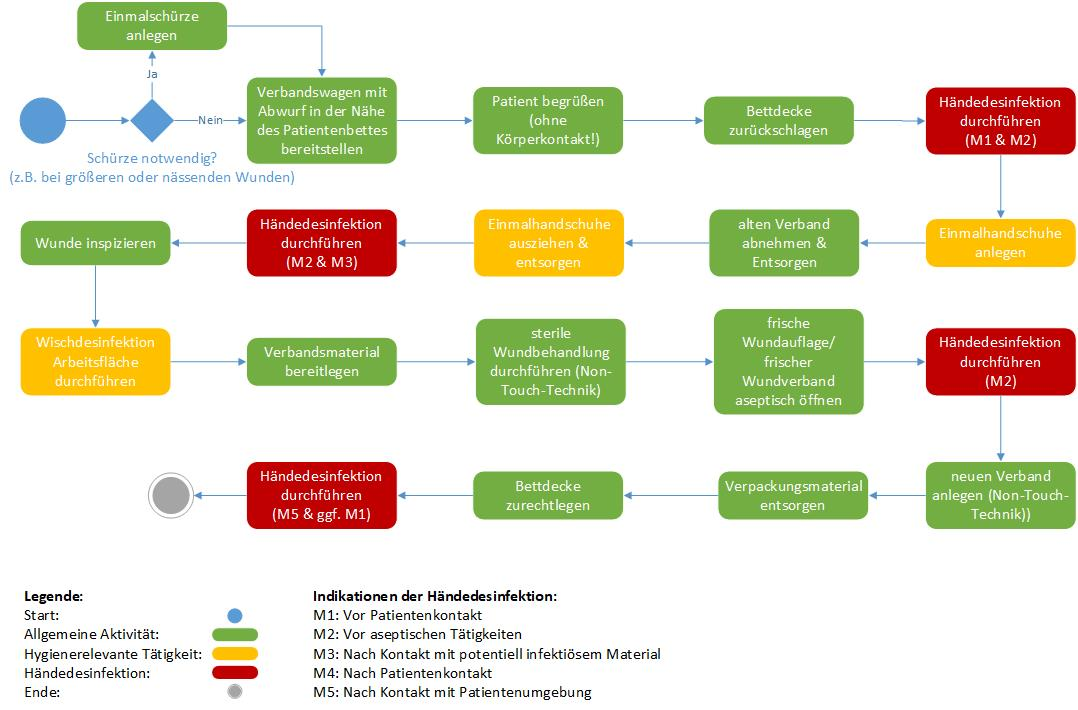
\includegraphics[scale=0.5]{img/Ablaufdiagramm_Verbandswechsel.jpg}
  \caption{Ablaufdiagramm Verbandswechsel \cite{AblauffdiagrammVerbandswechsel}}
  \label{fig:Ablaufdiagramm Verbandswechsel}
\end{figure}

Nun war die Aufgabe herrauszufinden, welche Möglichkeiten es gibt, diese Aktionen, die per EGO-Perspektiv-Video der Hololens aufgenommen wurden, zu erkennen. Die Wichtigsten Actionen sind hierbei das Desinfizieren und anlegen der Handschuhe. \ref{fig:Ablaufdiagramm Verbandswechsel}
Hierfür soll ein \acf{KNN} zuhilfe gezogen werden, welches die wichtigen Aktionen erkennt und somit die Fehlerquote, welche durch Vergessen oder Zeitstress entstehen, zu reduzieren. Dazu muss erst ein  Netz, welches für unser Anwendung passt, gefunden und für die oben genannten Anwendungen getestet werden, desweiten muss hierfür ein Datenset mit diesen Aktionen erstellt werden, welche zum Trainieren und Zesten des Netzes notwenig sind. Anschließend soll das Netz noch evaluieren und Verbesserungen vorgenommen werden.

\section{Grundlagen}
\label{sec:Grundlagen}
In diesem Kapitel werden die theoretischen Grundlagen, die zum Verständnis, der vorliegende Arbeit wichtig sind beschrieben. Zubeginn erfolgt eine kurzer einstieg in die Optimierungsgrundlagen. Dann folgt die Einführung in die Grundlagen der genetischen Algorithmen. Anschließend werden die wichtigen Grundlagen der Künstlichen neuronalen Netzen erklärt. Zum Schluss wird kurz auf die Hyperparameter eingegangen.

\subsection{Optimierungsgrundlagen}
Angenommen es soll ein Künstliches Neuronales Netz mit k Layern und L Neuronen zur Klassifizierung von einfachen handgeschriebenen Zahlen erstellt werden. Der Entwickler entscheidet sich für ein 3 Layern Netz mit jeweils 3 Neuronen. Nach dem Training hat es die Genauigkeit von 85 Prozent. Ist dies Akzeptabel? Kann man sagen, das für k = 3 bzw. j = 3 die optimale Lösung gefunden wurde? Um dies zu beurteilen müssen viele Experimente durchgeführt werden. Die Frage ist, wie man den die besten Werte für k und j finden um die Klassifizierung zu maximieren. Dieser Vorgang wird als Hyperparameter-Optimierung bezeichnet. Bei der Optimisierung wird mit einem Inizialwert gestartet dieser ist in den seltensten Fällen die exacte Lösung. Dieser Inizialwert muss einige male verändert werden um auf einen Optimum zu kommen. Manchmal ist dieses Anpassen/optimieren so Komplex, dass es durch eine Funktion ersetz werden muss.


\subsection{Genetische Algorithmen}

Die Inhalte des folgenden Abschnittes sind, sofern nicht anderweitig angeführt aus den Gurndlagen büchern xxxx und xxxx übernommen. 

Genetische Algorithmen sind heuristische Suchansätze. Im wesentliche zeichnet sie eine probabilistische Eltern Selektion als primären Suchoperator aus. Als Weitern Suchoperator kann noch auf die Mutation zurückgegriffen werden, dieser garantiert eine Erreichbarkeit aller Punkte im Suchraum und erhält die Grunddiversität in der Population. Es gibt zwei verschiedene Algorithmen der Standart-GA tauscht nach einer Generation die komplette Elternpopulation durch die Kinderpopulation aus. Und bestehen in der Regel immer aus fünf gleichen Schritten wie in Abb. \ref{fig:Ablauf_kurz} zusehen ist. Im Gegensatz dazu gibt es den Steady-State-GA welcher durch seine überlappende Population auszeichnet, dieser Algorithmus wird in der Arbeit nicht verwendet und wird deswegen nicht weiter erklärt. 

\noindent%
\begin{figure}[H]
  \centering  
  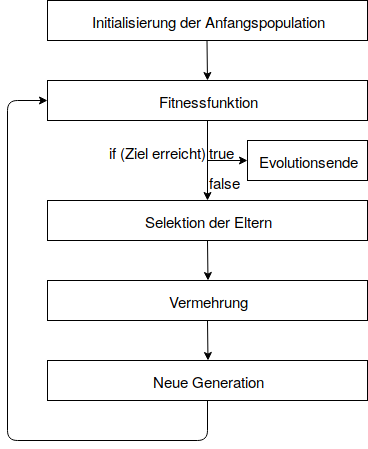
\includegraphics[scale=0.5]{img/Ablauf_kurz.png}
  \caption{Ablaufdiagramm eines Genetischen Algorithmuses mit 5 Schritten}
  \label{fig:Ablauf_kurz}
\end{figure}

Der Standard genetische Algorithmus \ref{fig:Ablauf_kurz} besteht aus folgenden 5 Schritte:
Schritt 1, Initialisieren einer Population.
Schritt 2, Fitness berechnen mit Hilfe der Fitnessfunktion.
Schritt 3, Selektieren der Eltern.
Schritt 4, Vermehren durch Cross-over und Mutation.
Schritt 5, Austausch der Populationen.
In den nachfolgenden Unterkapiteln werden auf die einzelnen Schritte genauer eingegangen. 

\iffalse
oder 

Der Standart Genetische Algortithmus \ref{Alorthm 1}besteht meist aus immer den gleichen Schritte:
Schritt 1 Inizialisieren einer Population.
Schritt 2 Fittness brechnen mit hilfe der Fitnessfunktion.
Schritt 3 Evolution (Weiterentwicken), hier werden zuerst die passenden Eltern ausgesucht und anschließend mit Crossover und Mutation die Kinder Population erstellt. 
Schritt 4 Elternpopulation durch die neue Kinderpopulation ausgetauscht.
Hier noch einamal als Pseudocode.


Algorithm 1 Basic Genetic Algorithm \\
1: initialize population \\
2: repeat \\
3: 		repeat \\
4:			fitness computation \\
5:			parent selection \\
6:			breed \\
7:		until population complete \\
8:		selection of parental population \\
9: until termination condition \\

Im nachfolgenden Unterkaptitel wird auf diese einzelnen Schritte genauer eingegangen.

\fi

\iffalse
Genetische Algorithmen sind im Wesentlichen durch eine probabilistische Eltern selektion und die Rekombination als primären Suchoperator gekennzeichnet.Die Mutation ist meist nur ein Hintergrundoperator, der mit einer geringen Wahrschenlichkeit zur anwendungkommt. Er garantiert die Erreichbarkeit aller Punkte im Suchraum und erhält eine Drunddiversitöt in der Population.

Evolutionäre Algo -- s.128


Genetische Algorithmen sind heuristische Suchansätzem, die auf einer breitenbasis von Optimierungsproblemen angewendet werden können. Diese Flexibiliät macht sie für die Praxis für viele sehr attraktiv.Die Evulution ist Grundlage des Genetischen Aglorithmuses. durch die aktuelle Vielfalt und der Erfolg der Arten ist dies schon alleine ein guter Grund sich diesen Optimierungs Algortihmus näher anzuschauen. Denn sdiese Arten sind in der lage sich an ihre Umgebung anzupassen und sich zu zu komplexen Strukturen zuentwickelen, und somit das überleben in verschiedesten Umgebungen eröglichen. Hierbei ist die Paarung und Entwicklung von Nachkommen eine der Hauptprinipen des Erfolges der Evolution. In diesem Kapitel werden wir die Grundlage der GEnetischen Algorithmen näher anzuschauen. Beginnen wir mit der grundlage das es sich bei den Genetischen Algorithmen um einen Polulations ansatz handelt. Anschließend wird auf die wichtigesten genetischen Operatioren vorstellen darunter gehöhren, Selektion, Crossover und Muttation

Seite - 11 Genetic Algorithm Essentials


Algorithmus 1 zeigt den Pseudocode des grundlegenden genetischen Algorithmus, der Folgendes kann dienen als Blaupause für viele verwandte Ansätze. Am Anfang eine Reihe von Lösungen,die als Population bezeichnet wird, wird initialisiert. Diese Initialisierung wird empfohlen.um zufällig den gesamten Lösungsraum abzudecken oder um Experten zu modellieren und einzubinden. Wissen. Die Darstellung bestimmt den Initialisierungsprozess. Für BitfolgeDarstellungen ist eine zufällige Kombination von Nullen und Einsen sinnvoll, z.B.das anfängliche Zufallschromosom 1001001001001 als typische Bitfolge der Länge 10. Der Hauptgenerationskreislauf des Genetischen Algorithmus erzeugt neue Nachkommen.Kandidatenlösungen mit Crossover und Mutation, bis die Bevölkerung vollständig ist.

Algorithm 1 Basic Genetic Algorithm
1: initialize population
2: repeat
3: 		repeat
4:			fitness computation
5:			crossover
6:			mutation
7:			phenotype mapping
8:		until population complete
9:		selection of parental population
10: until termination condition

Seite - 11 Genetic Algorithm Essentials
\fi 

\subsubsection{Aufbau und Initzialisierung einer Population}
Der klassische genetische Algorithmus basiert auf einer Reihe von Kandidatenlösungen. Die Größe der Population ist somit auch die Anzahl der Lösungen. Jede Lösung kann als einzelnes Individuum gesehen werden und wird durch ein Chromosomenstrang repräsentiert. Ein Chromosom besteht wiederum aus vielen Genen, welche die Parameter/hyperparameter repräsentieren. Der Aufbau ist grafisch in Figure \ref{fig:chromosome} gut zu erkennen. Es gibt verschiedene Möglichkeiten, diese Gene dazustellen. Wie Binär oder dezimal, um die Grundlagen nahe des später folgenden Konzepts zuhalten, wird der Ablauf per Dezimal-Genen erklärt.


\iffalse
Figure \ref{fig:chromosome} veranschaulicht ein Beispiel, wie eine Population aus vier Individuen(chromosomes)mit je einem Chromosom. Ein Chromso, besitzt wiederum  vier gene. Jedes dieser Gene ist durch eine binären zahl repräsentiert. 

\fi

\noindent%
\begin{figure}[H]
  \centering  
  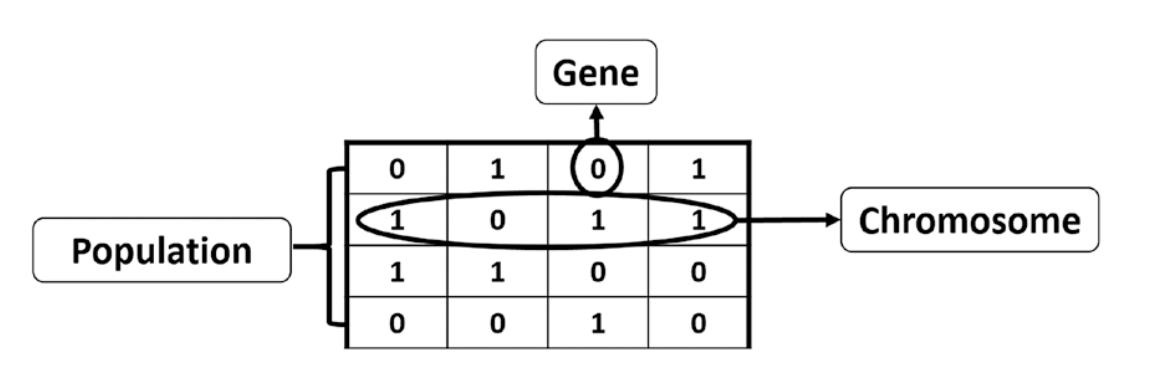
\includegraphics[scale=0.3]{img/Chromsome-s134-PracticalComputerVion.png}
  \caption{Beispiel einer Polulation mit 4 induviduen (Chromsomen) welche vier binäre Gene besitzen \cite{Rashid2017} }
  \label{fig:chromosome}
\end{figure}

Diese Anfangspopulation(Generation 0) wird zufällig initialisiert, um die größt mögliche Abdeckung des Suchraums zu gewähren. 

Die erste Generation besitzt (dadurch) eine sehr geringe Fitness, dies verbessert sich aber im Lauf des Trainings.
Die erste Generation besitzt eine sehr geringe Fittnes, welche im verlauf des Trainings stetig steigert bis sie das Maximum erreicht.

--- würde ich weglassen
Durch Selection werde die nicht unnötigen/Contra-produktiven Individumen oder auch Unfittesten Inidividuen aussotiert.
Dafür wird die Fittneswert benötig, welches im nächsten Punkt erklärt wird.
----


\subsubsection{Fittnesfunktion (eng. Fittnesfunction or grade)}
Die Fitnessfunktion bewertet das Individuum anhand seiner Funktionstauglichkeit, bezogen auf die vorhandene Aufgabe. Dabei werden nicht einzelnen Gene bewertet, sondern das ganze Genom/Chromosom/Individuum. Es gibt keine universelle Fitnessfunktion, diese muss also für jede Anwendung speziell geschrieben werden. Es wird also nicht berücksichtigt welches Gene sich positiv bzw. negativ auswirken. Als Rückgabewert gibt die Fitnessfunktion uns einen dezimalen/float Fitnesswert, dabei steht ein höherer Fitnesswert stehst für eine höher Qualität an Individuum sprich bessere Lösung.

\iffalse
Nun besteht die erste Generation(Generation 0) aus einer Population mit völlig zufälligen Induviduen. Es gibt keine universelle funktionierende Fitnessfuntion, diese muss für jeden Algorithmus neu geschrieben werden. Die Fittnesfunktion bewertet das Individum anhand seiner Funktionstauglichkeit bezogen auf die gestellte Aufgabe. Dabei werden nicht einzelnen Gene bewertet sondern das ganze Genom/Chromoson/Idividum. Es wird also nicht berücksichtigt welches Gene sich positiv bzw. negativ auswirken. Als Rückgabewert gibt die Fittnesfunktion uns einen Fittneswert, dabei steht ein höherer Fittnesswert stehts für eine höher Qualität an Individum sprich bessere Lösung.

Da nun alle Individuen der Population bewertet wurden kann eine neue Generation erstellt werden.

\fi


\iffalse
\subsubsection{Evolution (eng. Evolve) Fällt raus}

Bei dem Schritt Evulution geht es darum aus der Alten Population eine neue bessere Population zu erstellen. Dafür muss zu erst einen Elternpool (eng. matingpool), mit hilfe der eltern Selektion, erstellt werden. Aus diesem Elternpool wird mit Crossover und Mutation die neue Generation erstellt. 
Dazu  werden aus zwei Elternpaaren ein neues Kind erstellt.
Um die Elternpaare auszusuchen gibt es verschiedene Optionen. Da nun die Eltern fest stehen, wird per Crossover aus den beiden Elternpaaren oder aus dem Elternpool ein neues Kind generiert. Um bei den Genen eine höhere diversität zu gelangen werden die Kindergene noch mit einer Mutation versehen. Somit kann man einen höheren Suchraum(Abdeckungsgrad) abdecken. Nach dem eine neue Kind generation erstellt wurde wird der ganze vorgang so lange wiederhollt bis die geforderte Fintess ereicht wurde.

\fi

\subsubsection{Selektion der Eltern (eng. Select Parents)}
Bei dem Schritt Selektion geht es, darum einen Elternpool zu erstellen, aus welchem die neue Generation erstellt wird. Deshalb ist es wichtig, nur die besten, geeignetesten Individuen auszuwählen. Es gibt verschiedene Ansätze bei der Selektion, die bedeuteten werden genannt und erläutert.

Informationen wurden aus dem Paper \cite{shukla15} entnommen.


\begin{itemize}
\item \textbf{Auswahl proportional zu Fittnes (eng. Fitness Proportonal Selction(FPS))}, hierbei spielt die im vorigen Schritt berechnete Fitness eine große Rolle. Die Eltern werden nach ihrer Fitness proportional ausgewählt und zum Elternpool hinzugefügt. Wenn $f(a_i)$ die Fitness des Individuell $a_i$ in der Population ist, dann ist die Warscheinlichkeit selektiert/ausgewählt zu werden:
\begin{equation}
	ps(a_i) = \frac{f(a_i)}{\sum_{i=1}^n f(a_j)}; j\in{1,2,...,n} \label{eq:1}
\end{equation}
wobei n die Anzahl der individuen einer Population ist.
Diese Warscheinlichkeit $ps$ kann man sich, als Anteil auf einem Rouletterad, wie in Abblidung \ref{fig:roulette_wheel}, vorstellen. Auf dem dann Zufällig die Eltern aus den Idividuen a1,..,an "ausgedreht" werden.Problem hier ist das Individuen die am anfang gut sind schnell die ganz epopulation übernehmmen. Das kann dazuführen das eine mögliche bessere lösung durch den Algorithmus im suchraum nicht gefunden wird.

\begin{figure}[htb]
  \centering  
  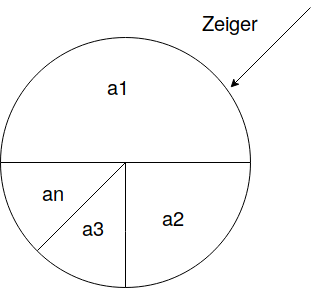
\includegraphics[scale=0.4]{img/roulette_wheel.png}
  \caption{Rouletterad mit Proportinalen Anteil der Individuen anhand ihrere Fitness}
  \label{fig:roulette_wheel}
\end{figure}


introduction to evolutionary comp s80

\iffalse
Problem hier ist das Individuen die am anfang gut sind schnell die ganz epopulation übernehmmen. Das kann dazuführen das eine mögliche bessere lösung durch den Algorithmus im suchraum nicht gefudnen wird. Ein weiteres Problem ist es wenn die Lösungen nahe bei bei einandern liegen gibt es fast keine selections druck mehr herscht. DIes geschied gegen ende der Optimierung und führt zu einem sehr langsamen verlauf gegen ende. 

introduction to evolutionary comp s80
\fi




\item \textbf{Ranking Selektion}, diese Selktion wurde von Backer als Verbesserung der Fitness Proportonal Selection entwickelt \cite{baker1985adaptive}. Dabei werden die Eltern nicht direkt nach ihrer Fitness ausgewählt. Die Fitness dient nur zum einteilen in eine Rangliste. Anhand dieser Rangliste wird dann wieder mit Hilfe des Rouletterades ausgewählt. Dabei gibt es verschiedene Verfahren wie diese Verteilung aussehen kann, einmal ein Lineare Ranking verfahren:
\begin{equation}	
	p_i = \frac{1}{N}(n^- + (n^+ - n^- ) \frac{i-1}{N-1}; i\in{1,...,N} \label{eq:2}
\end{equation}
Wobei $p_i$ die Warscheinlichkeit des i Idividums ist selektiert zu werden. $\frac{n^-}{N}$ ist die Warscheinlichkeit des Schlechtesten Indiviudums selektiert zu werden und  $\frac{n^+}{N}$ ist die Warscheinlichkeit des Besten Individums selektiert zu werden.

oder das expontienelle Ranking:
\begin{equation}
	p_i = \frac{c^{N-i}}{\sum_{j=1}^N c^{N-j}}; i\in{1,...,N} \label{eq:3}
\end{equation}
die Summe $\sum_{j=1}^N c^{N-j}$ normalisiert die Wahrscheilichkeit um sicherzustellen das $\sum_{i=1}^N p_i = 1$
Wobei die Berechnungen \ref{eq:2} und \ref{eq:3} nur den Anteil eines Individums auf dem Rouletterades verändern.

\iffalse
Sie werden nach ihrer Fitness sotiert und einem Rang Rk , k = 1, ...,N wobei N die anteil der individuen einer Population ist. Der beste kandidat erhält den besten Rang wobei der schrlechtestet den Rang N-1 erhält. Die fitness 

 Sie werden in einer Rangliste aufgestellt wobei das beste Individum den Rand y-1 belegt und das schlechteste den Rang 0. Dieses Ranking kann in vielen varianten vorgenommen werden, Linear oder expotenziel umgesetzt werden. 
\fi

\item \textbf{Tunier selektion}, in diesem Verfahren werden züfällig k Induviduen der Population ausgewählt. Diese k Induviuen  tretten wie in einem Tunier gegeneinander an. Der Gewinner ist das Individuum mit dem besten Fittneswert,dieser wird dann auch als Elternteil ausgewählt. Hierbei wird auf den Elternpool verzichtet und direkt ein Kind aus zwei Gewinnern erstellt. Eingesetzt wird dies bei kleineren Populationen mit weniger als 20 Individuen.

\begin{figure}[htb]
  \centering  
  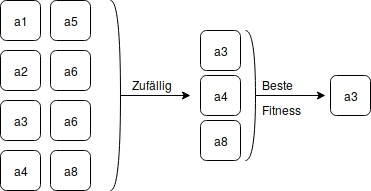
\includegraphics[scale=0.6]{img/Tunier.png}
  \caption{Tunier Selektion mit k = 3 Individuen und dem Gewinner Individuum 3}
  \label{fig:roulette_wheel}
\end{figure}


\end{itemize}


\subsubsection{Vermehrung (eng. Breed)}
Aus dem Elternpool/Paarungspool werden nun Nachkommen(Kinder) geschaffen. Alleine durch die Paarung(eng. Crossover) von qualitativ hochwertigen Individuen wird erwartet, dass die Nachkommen eine bessere Qualität besitzen als die ihrer Eltern. Als zweite Verbesserung wird noch die Mutation einzelner Gene angewendet. Für Crossover und Mutation gibt es verschiedene Ansätze, die in diesem Abschnitt genauer erklärt werden.



\iffalse
Dennoch kann es zu negative man nur die Eigenschaften der Eltern übernimmt kann es sogar dazu kommen das negative eigenschaften mit übernommen werden. Da dies natürlich nicht gewollt ist gibt es eine einfach Verbesserungs möglichkeit. Die Muation, hier wird jedes Gen noch einmal mit einer zufälligen Muation versehen welches ähnliche aber andere Lösungen hervorbringt. Nun gehen wir noch einmal genauer auf Operation Chrossover und Muation ein.

Somit müsste sich die Finttnes der nächsten generation verbessern. Um dies zu ereichen werden die  Gene noch modifiziert, durch corssover oder mutation. Somit wird der suchraum noch einmal vergrößert aber nur in der nähe der für gut empfunden Individuem bzw. dieser Gene.
Um aus den Einzelnen elternpaaren neue Individuen zu generieren wird das Verfahren/algorithmus Crossover verwendet. Bei Crossover kann es nun auch verschiedene möglichkeiten geben.
\fi


\paragraph{Crossover}, nennt man die Operation, bei der die Chromostränge der Kinder Individuen zusammengesetzt werden.
Beim Crossover gibt es mehrer Varianten, die One-Point-Crossover in welchem zufällig ein Punkt im Chromsomenstrang festgelegt wird.
Ab diesem Punkt wird der Chromosomenstrang dann aufgeteilt und anschließend mit dem Crossover des anderne Elternteils wieder zusammen gesetzt. Ein einfaches beispiel ist im Oberenteil der Abbildung \ref{fig:chromoson_crossover} zu sehen.

Eine Abwandlung des one-point-crossover ist das zwei-punkt-crossover oder k-point-crossover. Hier wird der Chromsomenstrang an k punkten aufgeteilt und anschließend wieder zusammengesetzt.
In mittleren Teil der Abbildung \ref{fig:chromoson_crossover}
ist ein k = 2 Crossover zu sehen.

Eine weite Grundlegende Operation beim Crossover ist die Uniformcrossover \cite{Syswerda1989} in welcher es keine Festgelegten punkte gibt. Hier wird für jedes Gen zufällig entschieden aus welchem Elternteil das Gen entnommen wird.
Dies im unteren Teil der Abbildung\ref{fig:chromoson_crossover} noch einmal veranschaulicht.

\begin{figure}[H]
  \centering  
  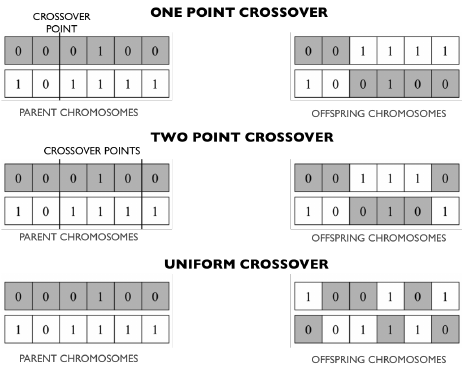
\includegraphics[scale=0.5]{img/Cossover.png}
  \caption{crossover anhand eines einfachen binären Chroms. Das erste zeigt eine 50/50 crossover. Das zweite zeigt eine Zufällige auswahl ders Gens.\cite{Rashid2017} }
  \label{fig:chromoson_crossover}
\end{figure}

Crossover nach dem Paper \cite{Umbarkar2015}.




\paragraph{Mutation},hierbei wird jedes Gen des Individuums zufällig mit einer zufälligen Mutation versehen. Durch diese Mutation wird eine höhere Diversität in die nachfolgende Generation übergeben. Diese Mutation macht es möglich einen größeren Suchraum abzudecken und somit die Werte genauer anzupassen, um so auf die Optimale Lösung zu kommen. 

\begin{figure}[H]
  \centering  
  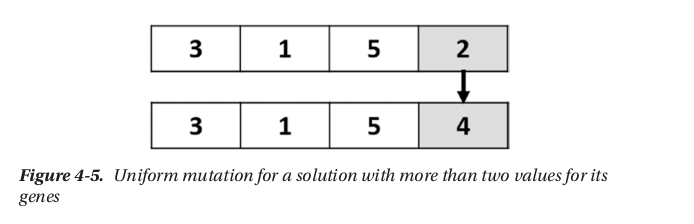
\includegraphics[scale=0.5]{img/mutation.png}
  \caption{Muation eines Genes um höhere vielfältigkeit zubekommen.\cite{Rashid2017} }
  \label{fig:chromoson_mutation}
\end{figure}


\subsubsection{Neue Generation}
Die neue Generation aus Kindern tauscht nun die alte Generation aus. Anschließend folgen die gleichen Schritte so lange bis die gewünschte Abbruchbedingung/ Fitnesswert erreicht ist. Aus dieser letzen Generation kann das beste Individum ausgesucht werden und als beste Lösung weiter verwendet werden. 

\newpage
\subsection{Künstliche Neuronale Netze}

Künstliche Neuronale Netze sind dem natürlichen Vorbild der neuronalen Netze im Gehirn nach empfunden. Beide Netze setzen sich aus einzelnen Neuronen zusammen, welche mit einandern verbunden sind. Wie man in Figure \ref{fig:neural_network} sieht ist jede Schicht ist aus einzelnen Neuronen aufgebaut welche mit den Neuronen der nächsten Schicht verbunden sind, diese Verbindungen repräsentieren die Gewichte, über diese kann einem Netz verschiedene Zusammenhänge von Input und Output antrainiert bzw. angelernt werden.

\begin{figure}[htb]
  \centering  
  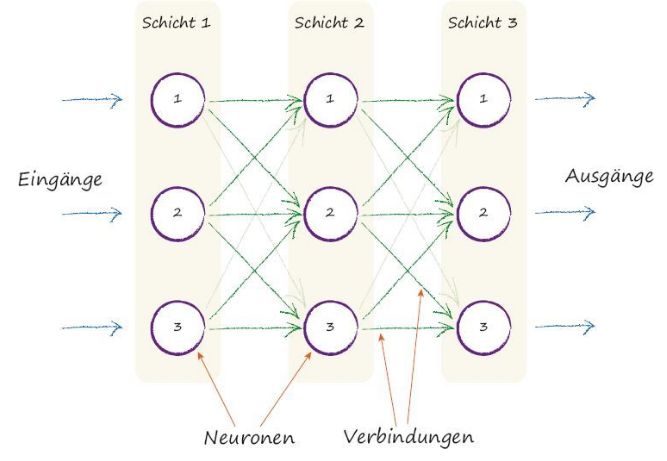
\includegraphics[scale=0.5]{img/S36_Buildyourown.png}
  \caption{Künstliches Neuronales Netz mit drei Schichten je drei Neuronen \cite{Rashid2017} }
  \label{fig:neural_network}
\end{figure}


Im folgenden Kapitel wird zuerst der Aufbau eines Neurons/Perseptron erklärt. Anschließend wird auf den strukturellen Aufbau eines Künstlichen Neuronalen Netzes nähergebracht. Zum Schluss werden noch wichtige Eigenschaften wie die Verlustfunktion und der Gradienten abstieg eingegangen sowie auf die Hyperparameter, welche für die Arbeit essentiell sind.



Grundlagen aus dem buch ArificalNeuroalNetworks s.11 


\subsubsection{Aufbau eines Neurons}



\begin{figure}[htb]
  \centering  
  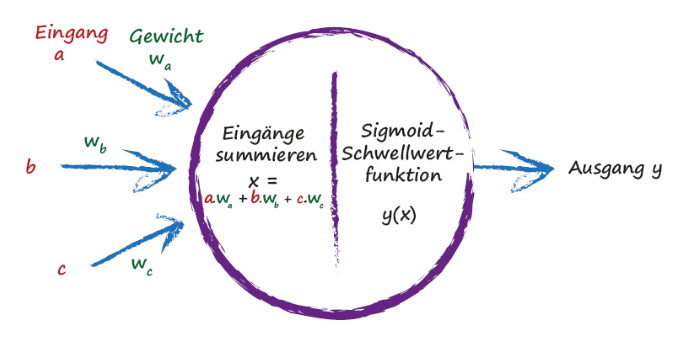
\includegraphics[scale=0.5]{img/S41_Buildyourown.png}
  \caption{Aufbau eines Neurons \cite{Rashid2017}}
  \label{fig:neuron}
\end{figure}

\paragraph{Eingang}
Bei dem Input handelt es sich um einfache xxxFloatwert dieser wird mit den einzelnen Gewichten verrechnet. Ein Neuron hat meist mehrere Eingangsgrößen, welche alle zusammen mit den Gewichten aufsummiert werden. Diese Werte werden zufällig initialisiert und per Training verbessert, somit handelt es sich um einen angelernten Werte, welche durch die Backproagation(Fehlerrückführung) verbessert werden.

\paragraph{Schwellwert aka bias}
Auf dieses Aufsummiertes Ergebniss wird anschließend ein Bias gerechnet, dieser führt zu einem besseren Verhalten beim Trainieren. Bei diesen Werten handelt es sich um angelernte Werte, die per Backpropagation verbessert werden und die Flexibitlität der Netze erhöht.


\paragraph{Aktivierungs Funktion}
Die Aktivierungsfunktion kann man sich als Schwellwert vorstellen, ab wann das Neuron den Input weiter gibt. Es gibt verschiedene Funktionen, um diesen Schwellwert zu definieren. Je nach Aufgabe des Neuronalen Netze werden andere Aktivierungsfunktionen verwendet. Bei Klassifizierungen werden heute meist ReLu-Layer oder ein Weakly-ReLu Layer benutzt, diese verhindern das Vanishing- bzw. Exploding- gradientproblem beim Trainieren.

\paragraph{Ausgang aka Output}
Wenn der Schwellwert überschritten wird, wird am Output durchgeschaltet. Dieser Output kann entweder mit einer nen Schicht Neronen verbundne sein oder direkt als Ausgang gesehen werden. Über welchen man anhand von xxxVariabelenwerten/Kommawerten die 
Von Input nach Output nennt sich ein Single-Forward-Pass. Wie hier beschrieben wird, kann ein Netz verschieden viele Layer besitzen mit verschiedenen Anzahlen von Neuronen.

\subsubsection{Struktureller Aufbau eines Neuronalen Netzes}

Wie kann ich Neuronen zusammenbauen usw.

\paragraph{Input Layer}

\paragraph{Hidden Layer}

\paragraph{Output Layer}

\subsubsection{Verlustfunktion aka lossfunktion}
Die Verlustfunktion stellt ein ausgesuchtes Maß der Diskrepanz zwischen den beobachteten und den vorhergesagten Daten dar. Sie bestimmt die Leistungsfähigkeit des neuronalen Netzes während des Trainings und der Ausführung. Ziel ist es, im laufenden Prozess der Modellanpassung, die Verlustfunktion zu minimieren.

\subsubsection{Optimierer alt Gradientenabstieg}
Um die Fehlerfunktion zu minimieren wird als Werkzeug der Gradienten Abstieg benutzt. Diese ist nur möglich da ein Künstliches Neuronales Netz aus verketteten differenzierbaren Gewichte der Neuronen(Tensoroperationen) aufgebaut ist, die es erlauben duch anwendung der Kettenregel die Gradientenfunktion zu finden, die den aktuellen Parametern des Datenstapels werte des Gradienten zuordnet. Es gibt auch hier verschiedene Ansätze von Optimierern, welche die genauen Regeln wie der Gradient der Verlustfunktion zu Aktualisierund der Parameter verwendet wird hier könnte Beispielweise den RMSProp-Optimierer, der die trägheit des Gradientenabstiegsverfahren berücksichtet.

Seite 83 - Deep Learning chollet


\iffalse
 Im Grunde werden dabei die Gewichte so angepasst, dass ein besseres Ergebnis entsteht und dadurch die Fehlerfunktion verringert wird. Wie das Wort Backpropagation schon sagt, wird von hinten nach vorne verbessert. Es gibt verschiedene Variationen von Gradientenabstiegen, welche verschiedene Vor- und Nachteile haben. Bei dem Trainieren des Netzes wurde der Momentum-Optimizer, welcher aus einem Gradientenabstieg mit Momentum aufgebaut ist.
\fi


\subsubsection{Hyperparameter}
Als Hyperparameter werden, in Bezug auf KNN's, meist die Anfangsbedingungen bezeichnet.
Für diese Hyperparameter gelten keine universellen Werte sondern müssen je nach Daten und Funktion bzw. künstliches Neuroales Netz speziell angepasst und verändert werden. Deshalb gibt es nur einige Regeln und grobe Abschätzungen in welchen grenzen sich diese Hyperparameter befinden. Zu diesen Hyperparameter gehören folgdende:
\begin{itemize}
\item \textbf{Learningrate},blabalaa
\item \textbf{Dropout}
\item \textbf{Lossfunktion}
\item \textbf{Optimizer}
\item \textbf{Model Achitektur}
\end{itemize}

\iffalse
Als Hyperparameter werden, in Bezug auf KNN's, meist die Anfangsbedingungen bezeichnet.
Dabei handelt es sich um die Learnrate (eng. Learningrate), der Abdeckunggrad(eng. Dropout), die Verlustfunktion oder auch der Optimizer. In selten Fällen kann die selbst Modelachitektur als Hyperparameter bezeicht werden. Für diese Hyperparameter gelten keine universellen Werte sondern müssen je nach Daten und Funktion bzw. künstliches Neuroales Netz speziell angepasst und verändert werden. Deshalb gibt es nur einige Regeln und grobe Abschätzungen in welchen grenzen sich diese Hyperparameter befinden. 
\fi


\subsection{Zusammenfassung}





\iffalse
Genetische algorithms ist ein sehr erfolgreiches Oprimiungsverfahren welches es erlaubt auch bei schweren Suchräumen lösungen zu finden. Insbesondere wenn keine gradienten berechnet werden können. In diesem Kapitel wurden die Grundlagen der genetischen Grundlagen zusammengefasst. Sie bassieren auf einer Lösungspopulation, die sich im laufe der iterationen dem Optima annähert. Genetische Operatioren ändern die Lösungen. Cross-overoperatoren kobinieren genome zweier Lösungen. Die Mutation fügt den Lösungen Zufälligkeiten hinzu und sollte somit jenden Ort im Lösungsraum erreichen. Der Genotyp oder Das Chromosom einer Lösing wird auf einen Phänotyp, die reale Lösung, abgebildetet, bevor es mit einer Fintessfunktion ausgewertet werden kann. Diese Fittnesfunktion muss sehr sorgfällig ausgearbeitet werden, da sie einen entscheidenden einfluss auf die Suche hat. Die Lösungen mit der höchsten fittnes sind folglich die Eltern der nächsten generation. Sobald eine Generation eine bestimmte Fintess ereicht sprich genug Optimiert wurde ist die beste Lösung gefunden. Somit wurde ein Algorithmus vorgestellt welcher auf ein breites Spektrum von Probkemen anwendbar ist.

Genectic - algorhmen - essential s.19 
\fi


%\chapter{Tätigkeitsbericht}
\label{chap:Taetigkeitsbericht}


\section{Chronologischer Tätigkeitsabriss}
\label{sec:Chronologischer_Taetigkeitsabriss}
\begin{figure}[htb]
  \centering  
  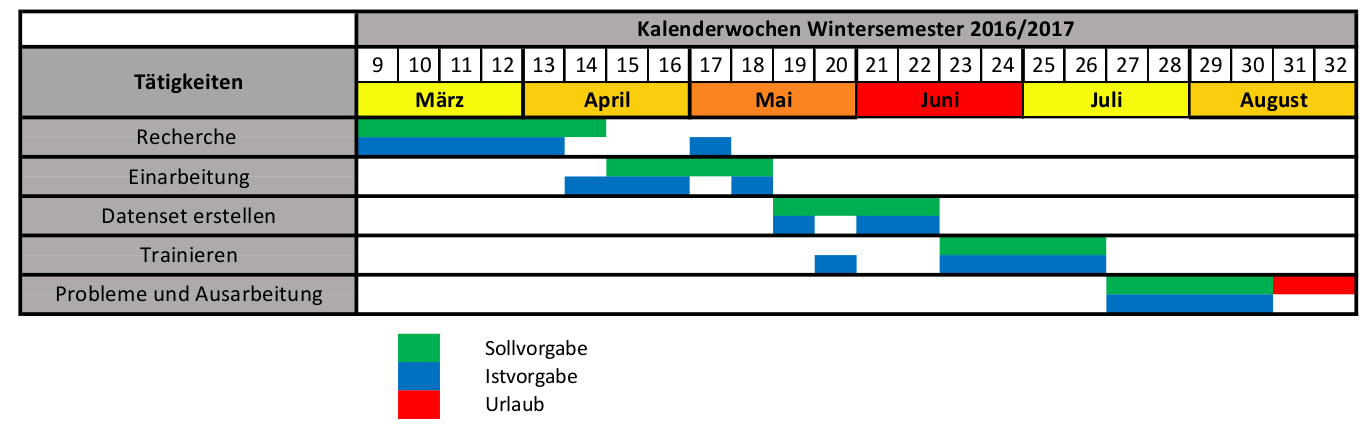
\includegraphics[scale=0.35]{img/GANTT-Diagramm.png}
  \caption{GANTT-Diagramm \cite{Gantt}}
  \label{fig:GANTT-Diagramm}
\end{figure}


\section{Internetrecherche}
\label{sec:Recherche}
Zu Beginn des Praktikums hatte ich wenige Vorkenntnisse in Action-Recognition und mit welchen Künstlichen Neuronalen Netzen man dies Umsetzen kann. Deshalb habe ich eine recht lange Recherchephase eingeplant, um mich mit dem Grundlagen des Thema ausführlich zu befassen. Es stellte sich heraus, dass es verschiedene Ansätze zur Actions-Recognition gibt:

\begin{itemize}
\item LSTM (Long- Short- Time Memory)
\item 3D Convolutional Networks
\item Two Stream 3D Convolutional Networks
\end{itemize}

Es gab viele Informationen und etliche Papers zu diesem Thema. Im Paper Quo Vadis, Action Recognition? A New Model and the Kinetics Dataset \cite{DeepMind/i3d} von GoogleDeepMind. Sie stellten verschiedene Ansätze nebeneinander und verglich welche Möglichkeiten sich als effektiv herausstellten. Das beste Netz dieses Papers war das Two-Stream 3D-Convolutional Netz, welches die besten Ergebnisse lieferte. Von Deep Mind wurde das Framework für dises Netz über Github frei zugänglich gemacht.

\section{Einarbeiten in vorhandene Frameworks}
\label{sec:Einarbeiten}
Die Einarbeitung gestaltete sich schwieriger als zuerst angenommen, da keine Funktionen zum Trainieren und Testen mitgeliefert wurden. Als Programmiersprache wurde Python benutzt und wie für DeepMind klassich wurde, als Front-End Sonnet, welches on top on Tensorflow aufbaut. Desweiteren habe ich ein Opensource Projekt der University of Science and Technology of China gefunden, welche ein Github Reposetorie zur Verfügung stellten, welches es ermöglichte dieses Netz zu trainieren und zu testen und von mir für unseren Anwendungsfall angepasst werden konnte.

\begin{figure}[htb]
  \centering  
  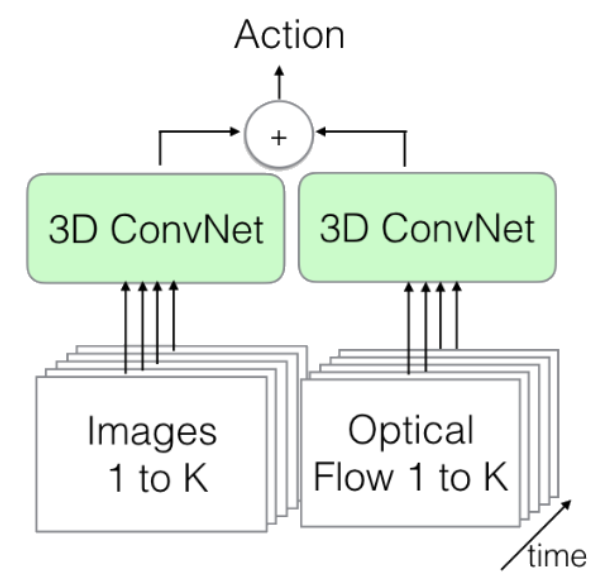
\includegraphics[scale=0.5]{img/Two-Stream.png}
  \caption{Two-Stream 3D-ConvNet  \cite{DBLP:journals/corr/CarreiraZ17}}
  \label{fig:Two-Stream 3D-ConvNet}
\end{figure}

Was heißt Two-Stream 3D-ConvNet?

Es handelt sich um zwei 3D-ConvNets. Eins für die Verarbeitung von RGB-Videos und eins für die Verarbeitung von Optical Flow Videos mit einer anschließenden Zusammenführung der Ergebnisse. Damit hat man stabilere Ergebnisse als nur einzelne Streams.

\newpage

\section{Optical Flow}
\label{sec:OpticalFlow}
Optical Flow ist die Bewegung von einzelnen Pixeln in X und Y Achse von zwei aufeinander folgende Frames eines Videos. Dieser Optical Flow wurde anfangs beiseite gelassen, um einen einfacheren Einstieg zu ermöglichen. Jedoch, zu einem späteren Zeitpunkt mit integriert. Um diesen Optical Flow zu extrahieren wurde von der Bibliothek Open-CV2 der Dense Optical Flow Alorythmus verwendet. Ich habe auch ein Künstliches Neuronales Netz das FlowNet2.0 \cite{FlowNet2.0} versucht für die Generierung des Optical Flow Images zu verwenden. Dies lieferte bessere Ergebnisse, dennoch war die Umsetzung zu Rechenaufwändig und somit für spätere Echtzeitanwendungen nicht brauchbar.

\begin{figure}[!htb]
  \centering
  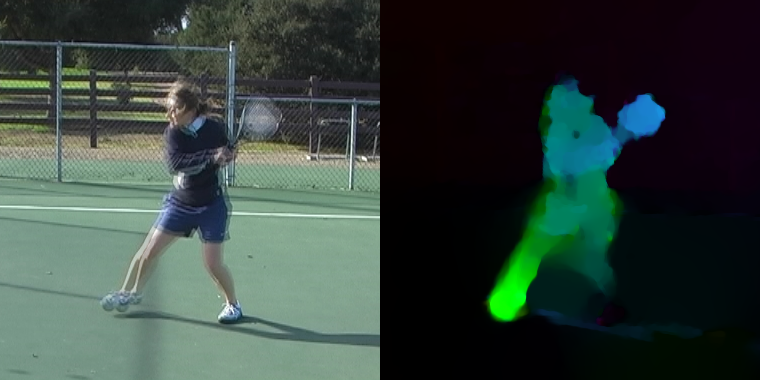
\includegraphics[scale=0.3]{img/tennis.png}
  \caption{Optical Flow   \cite{Bro11a}}
  \label{fig:Optical FLow}
\end{figure}

\section{Erstellen von Trainings- und Testdaten (Datenset)}
\label{sec:Datenset}
Ursprünglich wurde angedacht die Trainingsdaten mit der Microsoft Hololens zu erstellen. Da die Aktionserkennung auch für das Projekt mit der Hololens gedacht war. Dennoch stellte sich nach einigen Versuchen heraus, dass der Sichtwinkel der Hololence äusserst ungünstig ist und die Hände nur bei ausgestreckten Armen zu sehen sind. Dies ist aber keine natürliche Haltung. Um trotzdem ein Datenset zusammen zustellen wurde eine GoPro mit Kopfgurt benutzt. Welches mir es ermöglichte die Arbeiten unter normalen umständen aufzunehmen. Es war wichtig, an verschiedenen Orten und mit verschiedenen Personen diese Videos aufzunehmen, um gute aber gewollte Varianz in den Trainingsdatenset zu bekommen. 80\% der Videos wurden im FZI aufgenommen und 20\% der Videos wurden in der Uni-Clinc Heidelberg aufgenommen. Natürlich wäre es am Besten gewesen Videos aus realen Verbandswechsel mit Patienten zu haben, dies war aber aus rechtlichen Gründen (Datenschutz) noch nicht möglich.

 Es wurden ein Datenset zu folgenden Klassen erstellt:
\begin{itemize}
\item Gloves on (Anziehen von Handschuhen)
\item Clean (Putzen/Desinfizieren der Ablage)
\item unpacking (Auspacken der Verschlossenen Materialen wie Plaster und Verband)
\item Gloves off (Ausziehen von Handschuhen)
\item Disinfekt (Desinfiziernen der Hände)
\item Other (Verschiedene Actionen aus der Egoperspektive)
\end{itemize}


\section{Trainieren eines 3D-ConvNets}
\label{sec:Trainieren}
Um ein Netzwerk dieser Größe zu trainieren werden große Rechenleistungen benötigt. Deshalb wurde das Netz von Googles Deepmind auf das ImageNet Datenset vor trainiert. Dies brauchte auf 11 Tesla GPUS mehrer Wochen Training. Dieses Netz kann dann fine-getuned werden, also auf unsere Anwendungen angepasst werden. Das Finetunen funktioniert wie folgt: man schneidet die letzten Fully Connectet Layer ab und trainiert diese dann auf seine eigenen Daten neu. Somit ist es möglich, ein Netz in kurzer Zeit mit wenig Daten zu trainieren und zusätzlich noch gute Ergebnisse zu erhalten.


Das Training mit den RGB-Videos funktionierte gut. Und ergab nach den ersten Versuchen gute Ergebnisse. Das Ganze wurde dann mit Optical Flow wiederholt, somit hat man zwei Netze die einmal RGB Images und Optical Flow Images Verarbeiten können. Diese Ergebnisse werden anschließen zu einer Aussage zusammengefasst. Diese kann man dann mit einem Evaluierungstest auswerten.


%\chapter{Ergebnisse}
\section{Ergebnisse der Actionserkennung}
\label{sec:ergebnisse}
Es wurde ein Datenset erstellt welches aus 80\% selbst aufgenommen Videos und 20\% Videos aus der Uni Clinc Heidelberg.


Es wurde ein Neuronales Netz zur Action Erkennung gefunden. Für dieses Netz wurden Python Skripte erstellt, welche die Trainingsdaten so vor verarbeiten, dass damit ein Netz trainiert werden konnte. Anschließend wurde das 3D-ConvNet mit 6 Klassen: Gloves on, cleaning, unpacking, Gloves off, disinfekt, others mit jeweils 40 Videos trainiert. Die Evaluation gab gute Ergebnisse aus, das Netz hat eine Pression von 90\% erreichen. Mit diesen Ergebnissen konnte man zeigen, dass es möglich ist diese Netzstruktur für Ego-Action-Recognition zu verwenden.


\section{Verbesserungsvorschläge und Zukunftsaussicht}
\label{sec:Verbesserungen}

\subsubsection{Erweiterung der Trainingsdaten}
Die Trainerdaten können noch erweitert werden, einmal mit Realen Daten und weitern Klassen.
Oder mit Data-Argumentation, in welcher man durch Drehen oder einbringen von Farben künstlich mehr Daten erstellt und somit eine bessere Erkennung zubekommen.

\subsubsection{Realtime-Anwendung}
Die Schnelligkeit muss verbessert werden und die API muss angepasst werden, um es als Realtimeanwendung umsetzen zukönnen.
Dies übersteigt aber die Zeit in meinem Praktikum und ist deswegen noch zu entwickeln.

\subsubsection{Optical Flow}
Der Optical Flow wurde umgesetzt, dennoch ist es möglich, diesen zu Verbessern, durch verschiedene Vorverarbeitungen z.b. Bildstabilisierungen. Dies ist nicht getestet worden, könnte aber zu Verbesserungen führen, um Hintergrundstörungen aus den einzelnen Images zu filtern.

\subsubsection{Dritter Steam mit Händen}
Des Weiteren könnte man das Netz mit einem dritten Steam erweitern, um so den Focus auf spezielle Details zu legen.

\begin{itemize}

\item \textbf{Segmentation der Hände:}
Mit der Segmentation der Hände wäre es möglich speziellen Focus auf die Hände zulegen oder auf Video abschnitte mit Händen.

\begin{figure}[!htb]
  \centering
  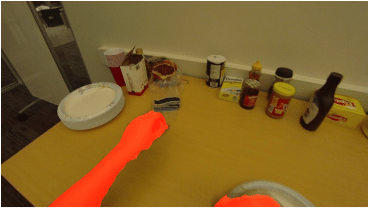
\includegraphics[scale=0.5]{img/hands.png}
  \caption{Segmentation Hands  \cite{Bambach_2015_ICCV}}
  \label{fig:Optical FLow}
\end{figure}

\item \textbf{Hand-Pose:}
Mit der Pose Estimation der Hände wäre eine Weiterentwicklung der Segmentation. Mit der Pose Estimation der Hände wäre eine Weiterentwicklung der Segmentation. Dennoch wurde dies meist mit RGB-D Images umgesetzt. RGB-D Images enthalten noch weiter Tiefeninformation welche die GoPro nicht mit liefert.

\begin{figure}[!htb]
  \centering
  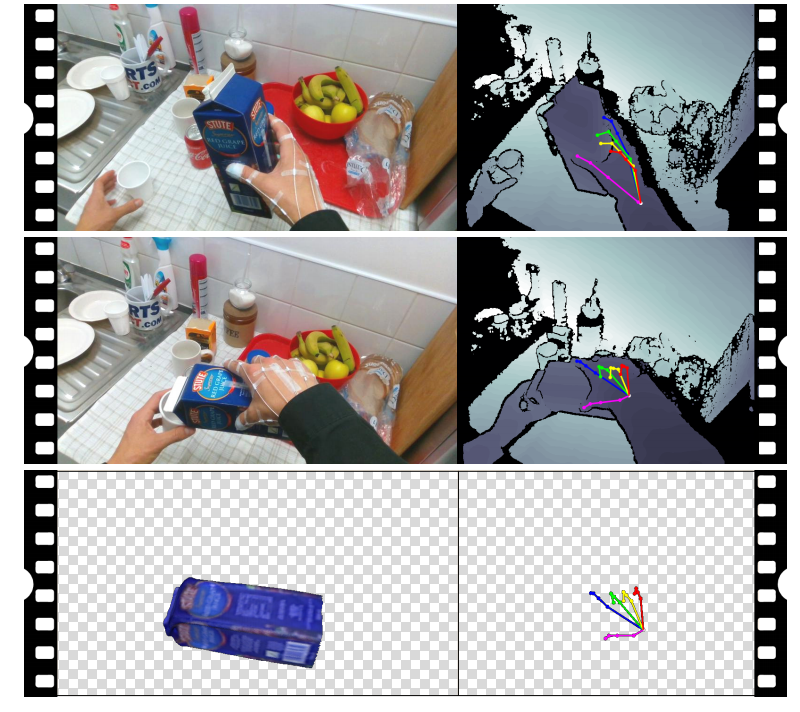
\includegraphics[scale=0.25]{img/Hand-Pose.png}
  \caption{Hand-Pose with RGB-D-Images   \cite{Hand-Pose-paper}}
  \label{fig:Optical Flow}
\end{figure}

\end{itemize}


%Literaturverzeichnis
\bibliographystyle{unsrtdin}
\bibliography{Literatur}

\end{document}
